\placelogofalse
\begin{frame}{OpenVDB}
\begin{columns}
\column{0.58\linewidth}
\centering
\begin{outline}
    \1 Originally from Dreamworks animation
    \1 Published in ACM Trans. Graphics
    \2 Describes VDB Datastructure
    \2 Introduced OpenVDB implementation
    \1 Widely used for special effects and animation
      \2 Supported by industry standard software like Houdini and Blender
    \1 Often used with implicit geometry
\end{outline}

\column{0.38\linewidth}
\centering
\shadowimage[width=2.5cm]{vdb_paper.png}
2013 \cite{Museth2013}\\
\vspace{0.5cm}
\includegraphics[width=4cm]{open_vdb_puss_in_boots.png} 
\end{columns}
\end{frame}
\placelogotrue

\begin{frame}{VDB Datastructure}
\begin{columns}
\column{0.38\linewidth}
\centering
\begin{outline}
    \1 Similar to B+Trees
    \1 Map based root 
      \2 Dynamic branching factor
      \2 Virtually infinite spatial bounds
    \1 Fixed height
    \1 Large (fixed) branching factors for children
\end{outline}

\column{0.58\linewidth}
\centering
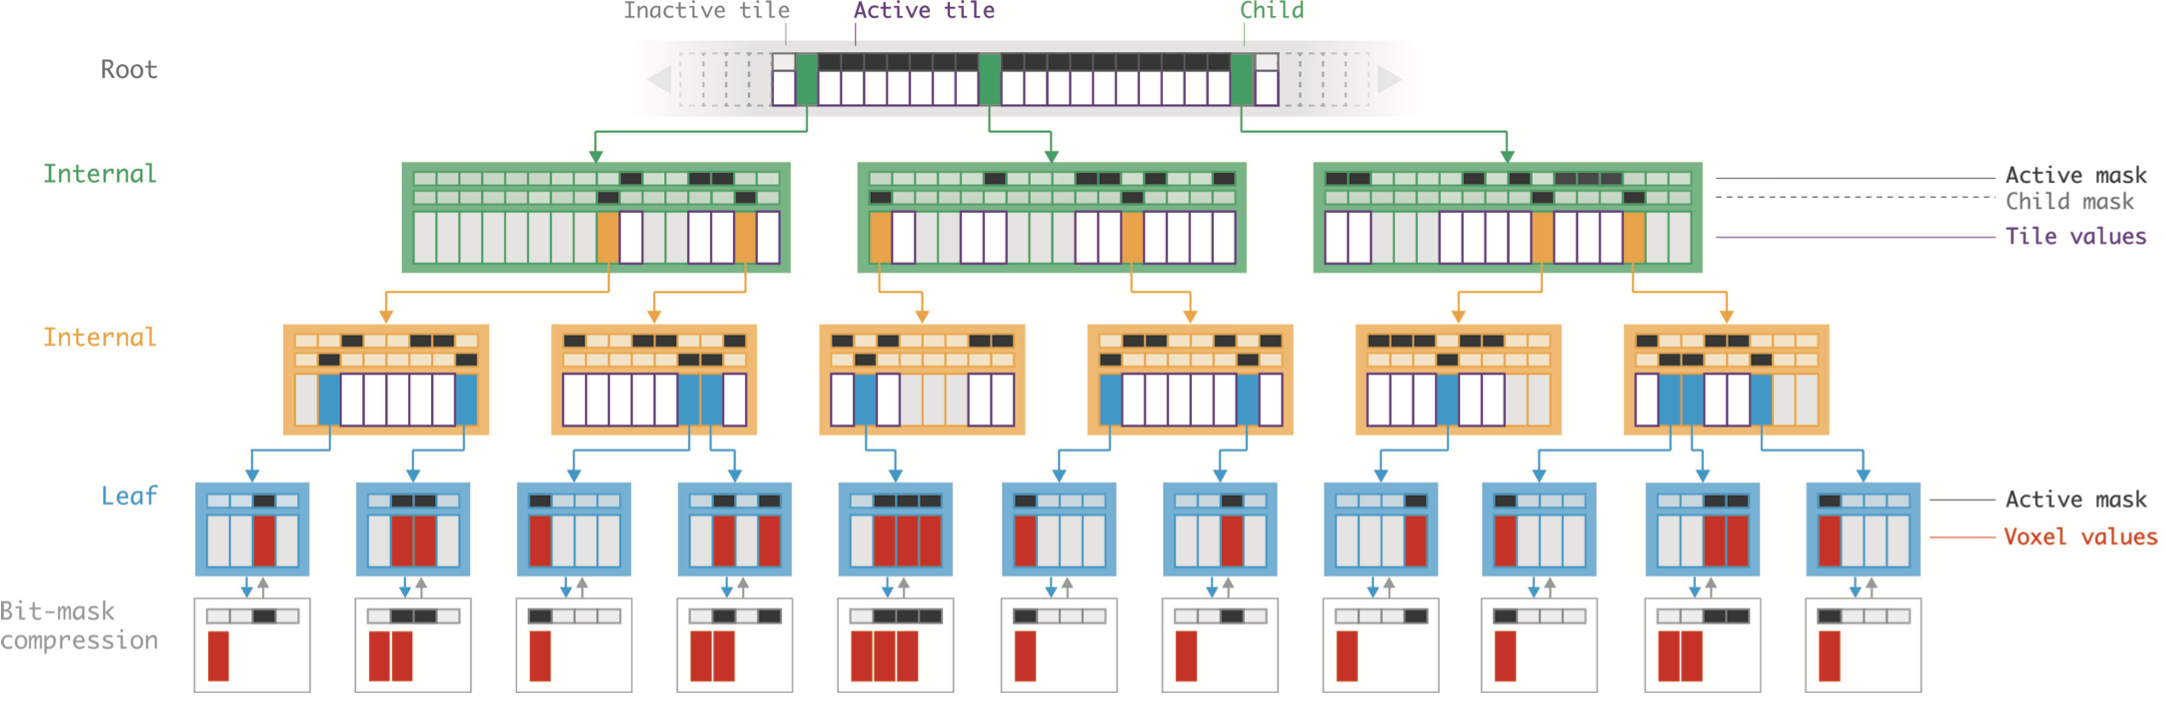
\includegraphics[width=7.0cm]{open_vdb_data_structure.png} \\
\vspace{0.5cm}
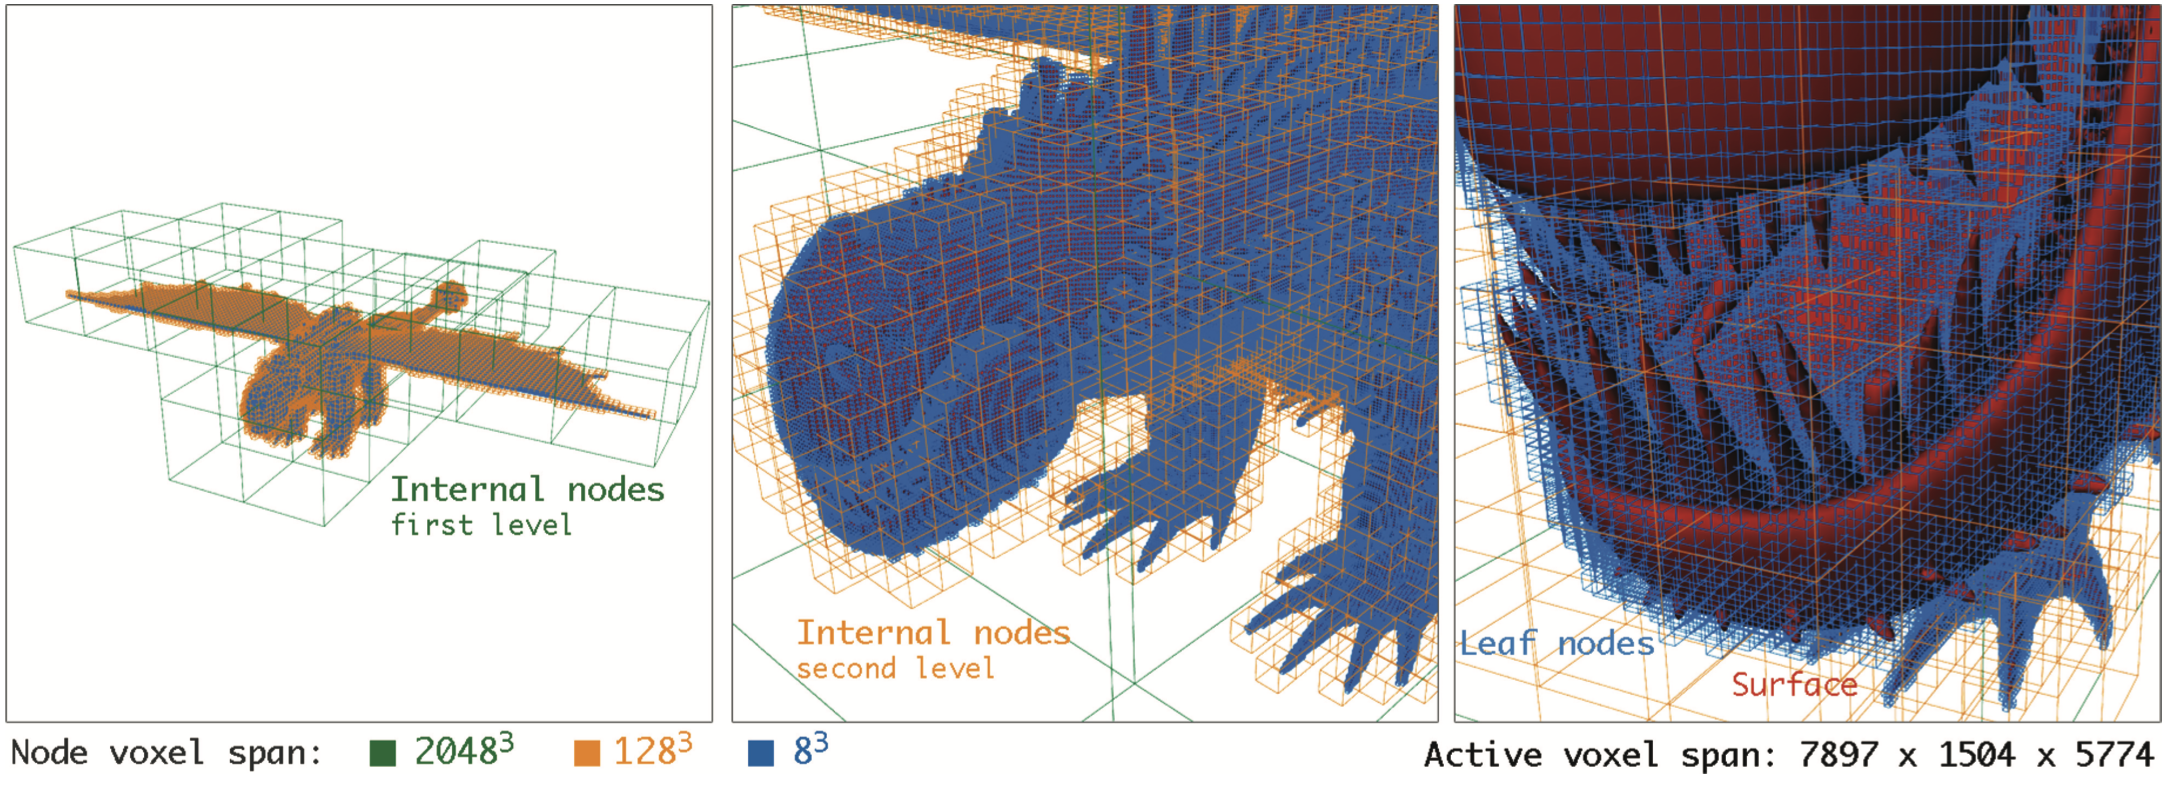
\includegraphics[width=7.0cm]{open_vdb_visual_aid.png} 
\end{columns}
\blfootnote{Images from \cite{Museth2013}}
\end{frame}
